\subsection{\decpomdp 정식화}
\label{sec:decpomdp_framework}

\Cref{fig:teaser}에 보인 것처럼, \bench의 \decpomdp에는 두 플레이어, 즉 에이전트와 사용자가 포함된다. 전체 과정은 튜플 $(\gS, \{\gA_i\}, \{\gO_i\}, \gT, \gR, \gU, \gM)$로 형식적으로 정의된다. 여기서 $i \in \{\agent, \user\}$는 플레이어를 나타내며, 튜플의 각 구성 요소는 아래에서 자세히 설명한다. 예시는 새 \telecom 도메인에서 가져왔다.

\textbf{메시지 공간 ($\gM$):} 에이전트와 사용자 사이에 교환될 수 있는 모든 가능한 (자연어) 메시지의 집합이다. 예를 들어 사용자는 ``I cannot use mobile data.''라고 말할 수 있고, 에이전트는 ``Could you check whether your airplane mode is on?''라고 응답할 수 있다.

\textbf{상태 공간 ($\gS$):} 전역 상태 $\gS = \gS_{world} \otimes \gS_{history}$이며, 여기서 $\gS_{world} = \gS_{db,\agent} \otimes \gS_{db,\user}$는 에이전트와 사용자의 \textit{기저} 데이터베이스 상태를 나타내고, $\gS_{history}$는 모든 상호작용 이벤트(행동, 관찰, 메시지)를 기록한다. 예를 들어 \telecom 도메인에서 $\gS_{db,\agent}$는 CRM 데이터(고객 프로필, 회선)일 수 있고, $\gS_{db,\user}$는 휴대전화 상태일 수 있다.

\textbf{행동 공간 ($\gA_i$):} 플레이어 $i$의 행동 $a_i \in \gA_i$는 도구 호출 $a_{i,tool} \in \gA_{i,tool}$ (\texttt{tool\_name(**kwargs)} 같은 함수 호출을 통해 $\gS_{db,i}$와 상호작용) 또는 메시지 $m_i \in \gM$ 중 하나다. 한 턴에는 한 플레이어만 행동한다. \telecom 도메인에서 에이전트는 \texttt{get\_customer\_by\_id(id)} 같은 도구에 접근할 수 있고, 사용자는 \texttt{toggle\_airplane\_mode()} 같은 도구에 접근할 수 있다.

\textbf{관찰 공간 ($\gO_i$):} 플레이어 $i$의 관찰 $o_i \in \gO_i$는 도구 관찰 $o_{i,tool}$ (예: $a_{i,tool}$에서 온 데이터, 메시지 또는 오류) 또는 플레이어 $j \neq i$가 보낸 메시지 $m_j \in \gM$ 중 하나다. 한 턴에는 한 플레이어만 관찰을 받는다. \telecom 도메인에서 에이전트는 \texttt{get\_customer\_by\_id}로부터 고객 세부 정보를 관찰할 수 있고, 사용자는 \texttt{toggle\_airplane\_mode}로부터 비행기 모드가 꺼졌음을 나타내는 메시지를 관찰할 수 있다.

\textbf{전이 함수 ($\gT$):} $\gT: \gS \times \gA \to \gS \times \gO$를 통해 시스템 동역학을 정의한다. 현재 상태 $s \in \gS$와 결합 행동 $a=(a_{\agent}, a_{\user})$가 주어지면, 새 상태 $s' \in \gS$와 결합 관찰 $o = (o_{\agent}, o_{\user})$를 산출한다. 도구 $a_{i,tool} \in \gA_{i,tool}$를 호출하면 $\gS_{world}$가 바뀔 수 있고 $o_i \in \gO_{i,tool}$가 산출될 수 있다. 메시지 $m_i \in \gM$를 보내면 $j \neq i$에 대해 $o_j=m_i$가 산출된다. 두 경우 모두 $s'$에는 갱신된 $\gS_{world}$와 $\gS_{history}$가 포함된다. 예를 들어 에이전트의 행동 \texttt{enable\_roaming(customer\_id, line\_id)}는 세계 상태(특정 회선 번호의 로밍 서비스가 활성화됨)를 갱신하고, 사용자의 행동 \texttt{toggle\_airplane\_mode}는 모의 휴대전화의 상태를 갱신한다.

\textbf{보상 함수 ($\gR$):} $\gR: \gS \to [0, 1]$인 함수로, 전체 상태 $s \in \gS$(데이터베이스 상태, 이력)에 기반해 전역 보상을 제공하여 과제 성공 또는 실패를 신호한다. 예를 들어 \telecom에서는 사용자의 데이터베이스 상태로 검증했을 때 사용자 문제("no mobile data")가 해결되면 에이전트가 보상을 받는다.

\textbf{지시 공간 ($\gU$):} 지시 공간 $\gU$는 현실적인 사용자 시뮬레이션을 안내하는 시나리오와, 사용자를 지원할 때 에이전트가 준수해야 하는 도메인 정책을 정의한다.

Dec-POMDP 정식화는 복잡하고 상호작용적인 시나리오를 시뮬레이션하는 데 핵심적인 장점을 제공한다(상호작용 궤적의 예시는 \Cref{fig:traj} 참조). 
이는 기술 지원처럼 사용자가 에이전트의 안내에 따라 도구 행동을 실행하는 협업 환경의 현실적인 시뮬레이션을 가능하게 한다. 이는 에이전트에게 중요한 조정 및 의사소통 과제를 제시한다. 
또한 이 정식화는 사용자 시뮬레이션의 신뢰성과 제어 가능성을 높인다. 사용자 도구와 그것이 사용자 상태에 미치는 효과를 정의함으로써 사용자 행동은 더 예측 가능해지고 광범위한 자연어 프롬프팅에 덜 의존하게 된다.

\begin{figure}[tb]
    \centering
    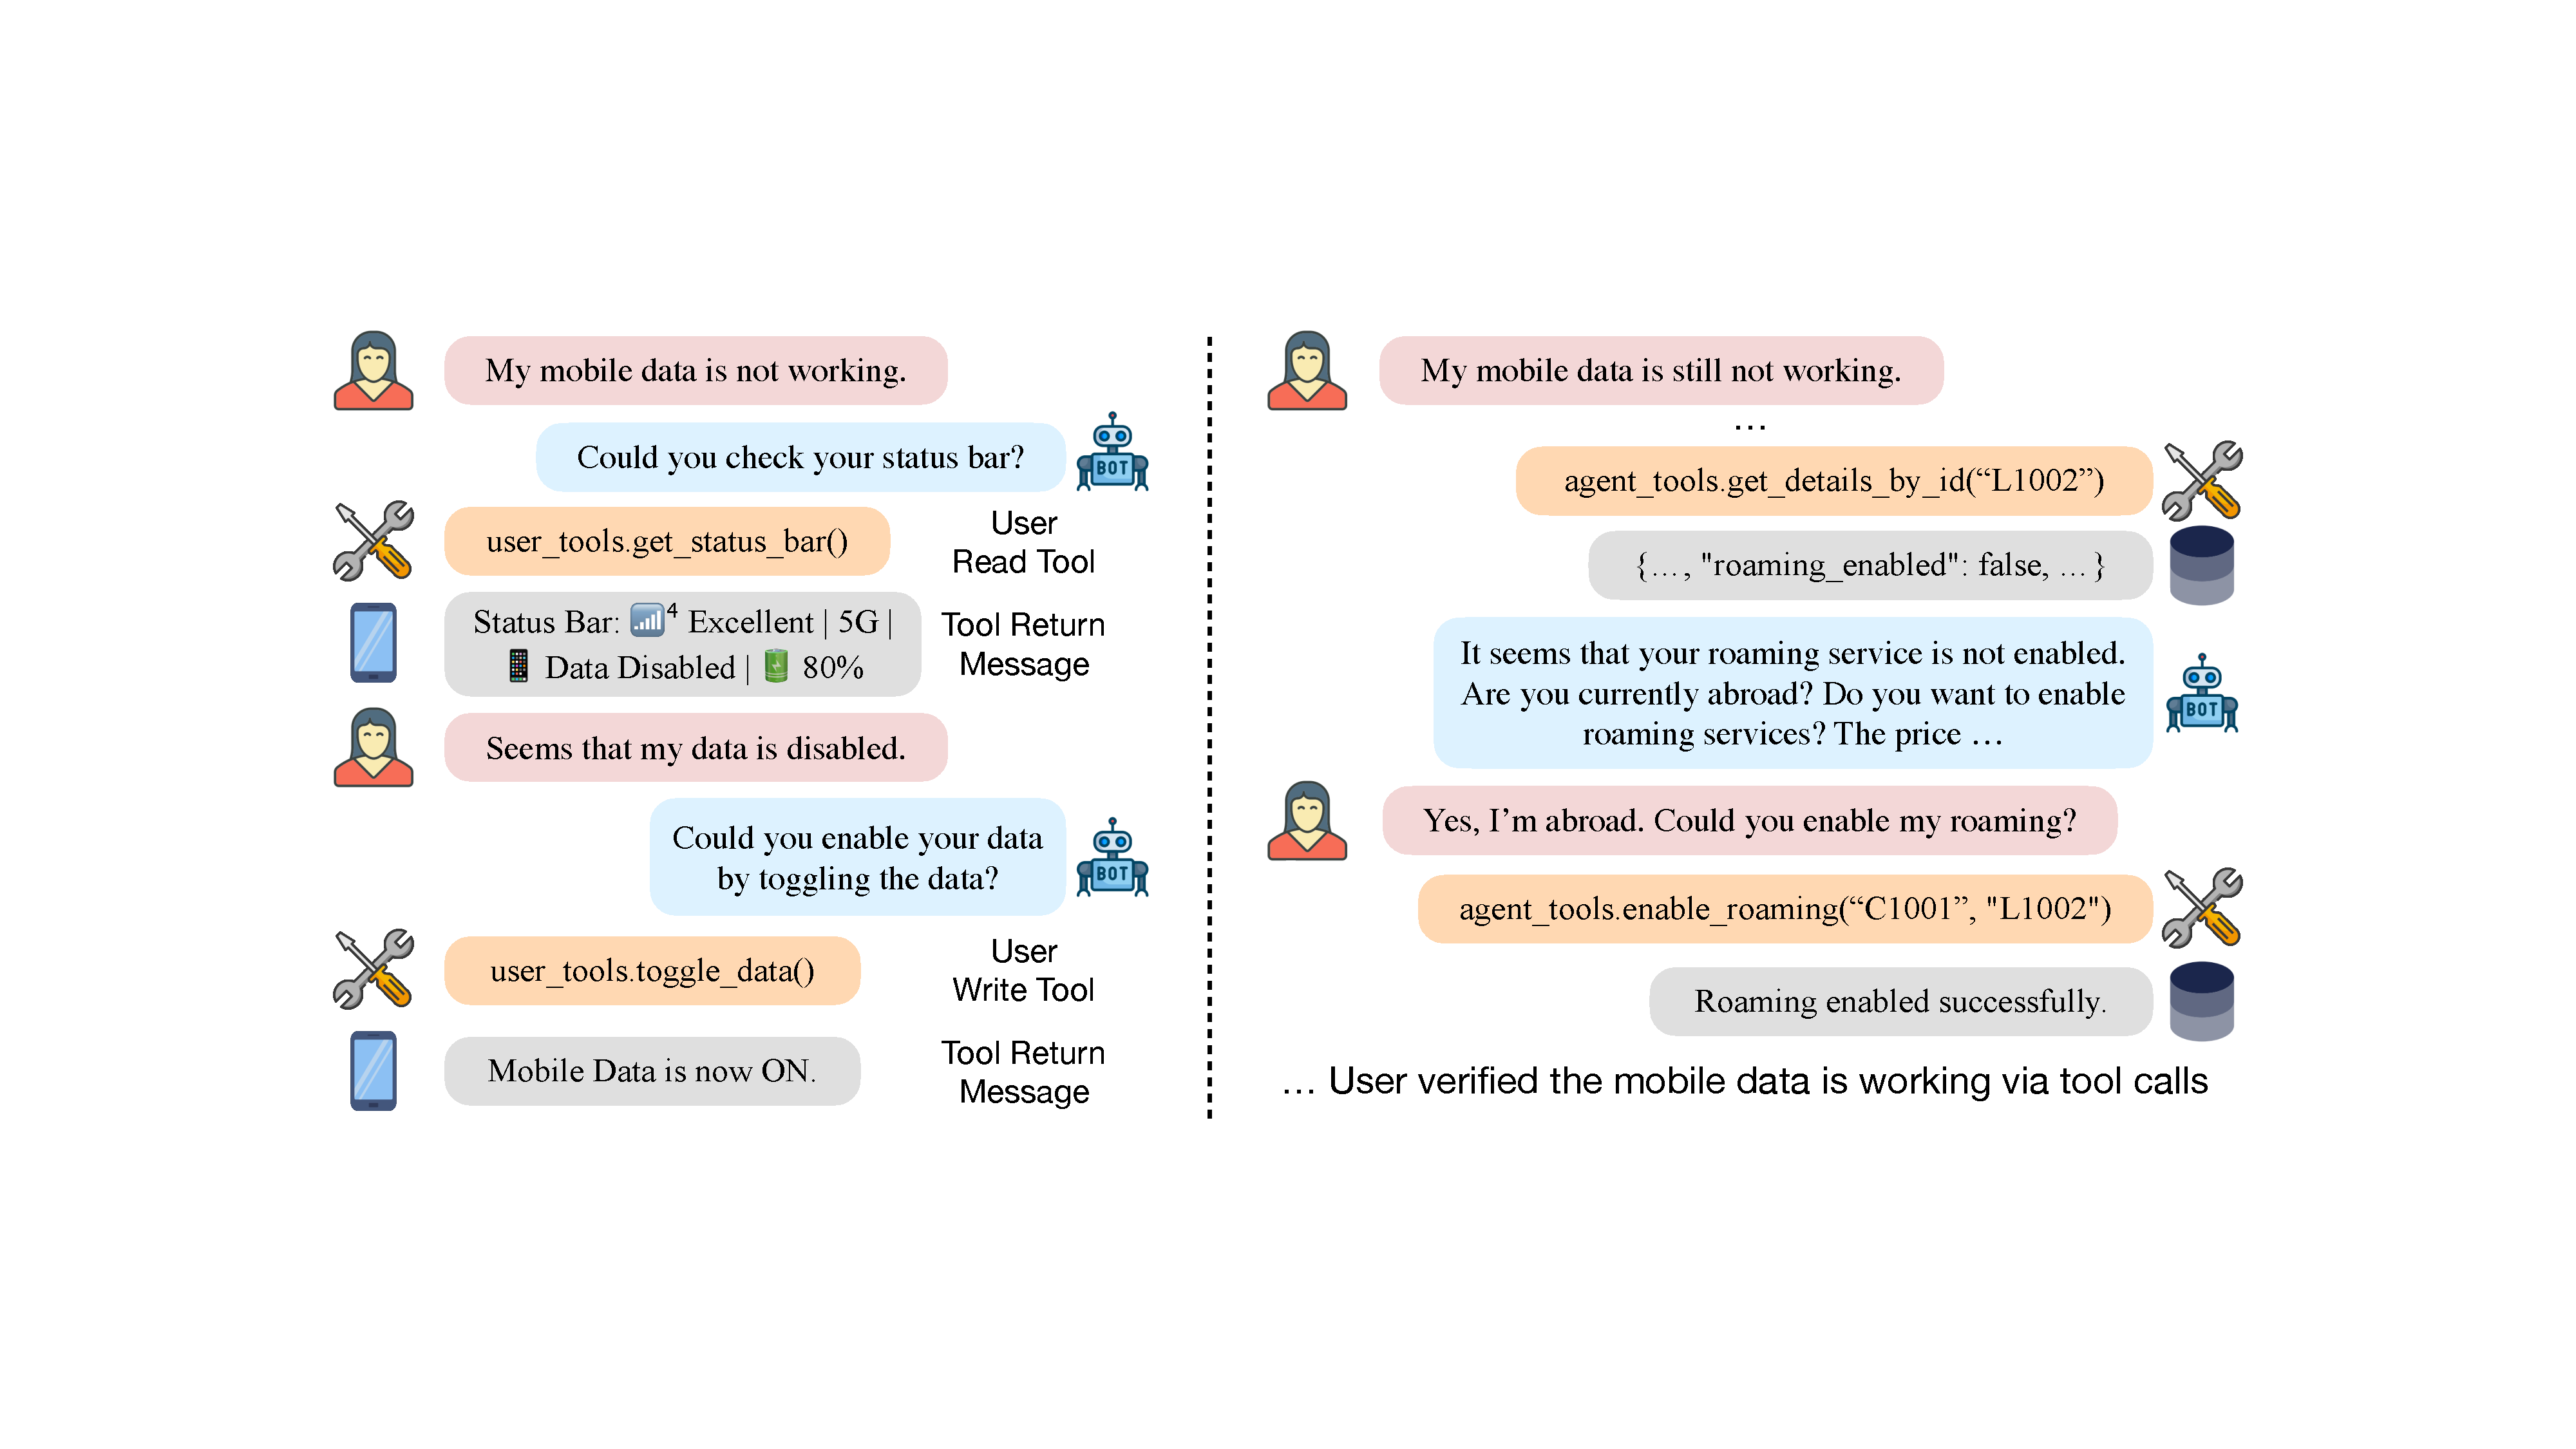
\includegraphics[width=0.99\textwidth,trim=240 240 240 240,clip]{figures/raw/traj.pdf}
    \vspace{-0.5em}
    \caption{\telecom 도메인에서 \bench의 에이전트-사용자 상호작용 trajectory($\gS_{history}$) 예시. 사용자 도구(모의 전화)의 구현을 제어함으로써, 기저 데이터베이스 상태를 바탕으로 ``상태 표시줄 확인''과 ``데이터 전환'' 같은 에이전트의 실행 가능한 지시에 대한 사용자의 응답을 안정적으로 시뮬레이션할 수 있다. 오른쪽 절반에서는 에이전트의 도구 호출이 사용자의 데이터베이스 상태에 미치는 영향을 모델링할 수 있음을 보여 주며, 여기서는 사용자에 대한 roaming 서비스가 에이전트 쪽에서 활성화되어 사용자의 전화가 roaming할 수 있게 된다.}
    \label{fig:traj}
\end{figure}


\subsection{도메인과 과제 생성}
\label{sec:curating_domains}

\begin{table}[t]
    \centering
    \caption{\bench 도메인의 핵심 통계.}
    \label{tab:domains}
    \vspace{0.2em}
    \begin{adjustbox}{width=0.95\textwidth}
    \begin{tabular}{llll}
    \toprule
     & \textbf{\retail{}} & \textbf{\airline{}} & \textbf{\telecom{}} \\
    \midrule 
    \textbf{에이전트 데이터베이스} & 사용자 500명, 제품 50개, 주문 1,000건 & 사용자 500명, 항공편 300편, 예약 2,000건 & 요금제 5개, 회선 9개, 고객 4명 \\
    \textbf{에이전트 도구} & write 7개, read 6개 & write 6개, read 6개 & write 6개, read 7개 \\
    \textbf{사용자 도구} & - & - & write 15개, read 15개 \\
    \textbf{과제} & 115 & 50 & 114 (full: 2285)\\
    \bottomrule
    \end{tabular}
    \end{adjustbox}
\end{table}


\taubench와 유사하게, 우리는 새 도메인에 대한 도메인별 자료를 구축하기 위해 다단계 생성 과정을 채택했다. \telecom 도메인을 예로 들면, 이 과정은 다음 단계로 이루어진다:

\textbf{1단계: 에이전트의 데이터베이스 스키마와 도구 생성.}
우리는 먼저 대규모 언어 모델(LLM)에 도메인의 핵심 비즈니스 로직을 개괄하는 제품 요구사항 문서(Product Requirements Document, PRD)를 생성하도록 프롬프트한다. 이 PRD는 데이터베이스 스키마와 필요한 함수를 명세한다. \telecom 도메인에서는 고객과 회선을 위한 스키마 및 이를 관리하는 함수를 갖춘 고객 CRM 시스템을 정의하는 일이 포함되었다. 그런 다음 LLM은 PRD에 기반해 함수 구현, 모의 데이터베이스, 단위 테스트를 생성한다. 우리는 모든 단위 테스트가 통과할 때까지 생성된 코드를 수동으로 정제한다.

\textbf{2단계: 사용자의 데이터베이스 스키마와 도구 생성.}
문제 해결 시나리오의 경우, 우리는 마찬가지로 LLM을 사용해 사용자의 데이터베이스 스키마와 도구를 정의한다. \telecom 도메인에서는 상태(예: 신호 강도)와 함수(예: 비행기 모드 토글)를 갖춘 모의 사용자 휴대전화 장치를 구현하는 일이 포함되었다. 여기서도 LLM은 구현, 모의 데이터베이스, 단위 테스트를 생성하고, 이후 모든 테스트가 통과할 때까지 이를 수동으로 정제한다.

\textbf{3단계: 프로그램적 과제 생성.}
우리는 원자적 빌딩 블록으로부터 다양하고 검증 가능한 과제를 생성하기 위해 조합적 접근을 사용한다.

각 원자적 하위과제 $t$는 해결해야 할 특정 문제에 관한 것이다. 예를 들어 비행기 모드가 켜져 있어 모바일 데이터가 작동하지 않는 경우가 있다. 구체적으로 각 하위과제 $t$는 $(\{f_{t,k}^{init}\}, \{f_{t,k}^{sol}\}, \{f_{t,k}^{assert}\})$로 정의된다. 여기서 $f_{t,k}$는 에이전트 또는 사용자의 데이터베이스와 상호작용하는 하위과제 $t$의 $k$번째 함수 호출이다:
\begin{itemize}
    \setlength\itemsep{0em}
    \item \textbf{초기화 함수 $f_{t,k}^{init}$}는 일반적으로 데이터베이스 값을 갱신하여 초기 과제 상태를 설정하는 호출을 명세한다. 예를 들어 \telecom에서 초기화는 \texttt{set\_airplane\_mode(True)}일 수 있다.
    \item \textbf{해결 함수 $f_{t,k}^{sol}$}는 초기화로 도입된 문제를 해결하기 위한 도구 호출을 명세한다. 예를 들어 \texttt{toggle\_airplane\_mode()}는 위에 제시한 초기화 예시에 대한 해결책일 수 있다. 이들은 에이전트나 사용자가 이용할 수 있는 도구여야 함에 유의하라.
    \item \textbf{검증 함수 $f_{t,k}^{assert}$}는 과제가 해결된 것으로 간주되기 위해 최종 상태 $\gS$가 만족해야 하는 조건을 명세한다. 예를 들어 \texttt{assert\_service\_status("connected")}는 \telecom에서 사용자의 서비스가 활성 상태인지 확인한다.
\end{itemize}

해결 함수 $f_{t,k}^{sol}$는 에이전트 또는 사용자 도구로 제한되지만, 초기화 및 검증 함수는 관련 데이터베이스의 어떤 함수도 될 수 있다.

원자적 하위과제는 상호 배타적이거나 대안적인 하위과제들이 같은 그룹에 속하도록 묶인다. 복합 과제는 각 그룹에서 최대 하나의 하위과제를 선택하고, 각각의 함수 호출을 이어 붙여 생성된다.
과제 정확성은 초기화 함수를 적용한 뒤 해결 함수를 적용했을 때 최종 상태 $s \in \gS$가 모든 검증 함수를 만족하는지 확인하여 자동으로 검증된다. 또한 모든 해결 함수가 적용되기 전에는 과제가 해결되지 않음을 검증한다.

\telecom 도메인에서 우리는 복잡도가 증가하는 3개의 사용자 의도, 즉 \serviceissue, \mobiledataissue, \mmsissue에 대해 15개의 원자적 하위과제 그룹을 개발했다.
이 하위과제들을 프로그램적으로 조합하면 2285개의 과제가 생성된다. 그런 다음 서로 다른 의도와 하위과제 수에 걸쳐 균형 잡힌 분포를 이루도록 114개 과제를 서브샘플링했다(자세한 내용은 \Cref{app:telecom}). 과제의 하위과제 수는 더 많은 진단 및 해결 단계가 필요하므로 난이도의 대리 지표로 쓰인다.


\textbf{4단계: 도메인별 에이전트 정책 생성.}
선별된 과제와 그 해결책에 기반해, 우리는 LLM에 에이전트를 위한 도메인별 정책을 생성하도록 프롬프트한다. 문제 해결의 경우 이러한 정책은 사용자 문제를 진단하고 해결하도록 에이전트를 안내하며, 각 사용자 의도와 관련된 일반적 문제에 대한 단계별 절차를 개괄하는 경우가 많다. 자세한 내용은 \Cref{app:telecom-policy}에 있다.

\textbf{5단계: 수동 정제.} 우리는 도구, 정책, 원자적 하위과제를 포함한 모든 도메인 자료를 공동으로 정제하여 도메인의 품질을 높인다.

또한 원래 \taubench와 비교해 \bench는 개발자가 과제를 페르소나(Persona, 사용자의 정체성에 대한 간단한 설명)와 구체적으로 연결할 수 있게 한다.
우리는 새 도메인에서 이를 활용했다. 각 \telecom 도메인 과제에는 다음 페르소나 중 하나가 무작위로 할당되었다: \texttt{None}, \texttt{Easy}, \texttt{Hard}. \texttt{None} 페르소나는 사용자 시뮬레이터에 특정 페르소나가 제공되지 않음을 의미한다. \texttt{Easy} 페르소나는 도메인에 상당히 익숙한 사용자의 프로필을 설명하고, \texttt{Hard} 페르소나는 기술 지식이 낮아 더 까다로운 사용자를 나타낸다(\Cref{app:telecom-user-persona} 참조).

\subsection{과제 평가}
과제 성공은 DB 검사, 상태 검증, 자연어 검증, 의사소통 정보 검사, 행동 매칭이라는 서로 다른 기준으로 정의될 수 있다.
DB 검사와 의사소통 정보 검사는 원래 \taubench와 동일하다. 상태 검증은 미리 정의된 검증 함수(예: 서비스가 연결되어 있는지 확인)를 사용해 최종 세계 상태 $\gS_{world}$의 특정 조건을 검증하는 것을 포함한다. 자연어 검증은 ``the agent diagnosed the cause of the issue.''와 같은 자연어 설명을 사용해 최종 이력 상태 $\gS_{history}$의 특정 조건을 검증하는 것을 포함한다. 행동 매칭은 실제 에이전트-사용자 상호작용 궤적 안에 모든 해결 함수 $f_{t,k}^{sol}$가 존재하는지 검증하는 것을 포함한다.
실제로 각 과제는 그 특징에 따라 이러한 기준의 부분집합을 명세할 수 있다. \telecom에서는 과제 성공을 평가하는 데 검증 함수만 사용한다.


